\documentclass[a4paper,11]{article} 
\usepackage[left=1in,right=1in,top=1.5cm,bottom=1cm]{geometry}
\usepackage{graphicx}
\usepackage{subcaption}
\usepackage{float}
\usepackage{listings}
\usepackage{color}
\usepackage{amsmath}
\usepackage{hyperref}

\graphicspath{{../data/}{../data/tracking-seg/}{../data/eval-data-gray/}}
\hypersetup{colorlinks=true,linkcolor=blue,urlcolor=blue}
  
\definecolor{codegreen}{rgb}{0,0.6,0}
\definecolor{codegray}{rgb}{0.5,0.5,0.5}
\definecolor{codepurple}{rgb}{0.58,0,0.82}
\definecolor{backcolour}{rgb}{0.95,0.95,0.92}
 
\lstdefinestyle{mystyle}{
    backgroundcolor=\color{backcolour},   
    commentstyle=\color{codegreen},
    keywordstyle=\color{magenta},
    numberstyle=\tiny\color{codegray},
    stringstyle=\color{codepurple},
    basicstyle=\footnotesize,
    breakatwhitespace=false,         
    breaklines=true,                 
    captionpos=t,                    
    keepspaces=true,                 
    numbers=left,                    
    numbersep=5pt,                  
    showspaces=false,                
    showstringspaces=false,
    showtabs=false,                  
    tabsize=4
}
 
\lstset{style=mystyle}
\pagenumbering{gobble}
\allowdisplaybreaks

\begin{document}

\begin{center}
  \large{\textbf{CSE578 Computer Vision}}\\
  \Large{\textbf{Assignment 5 : Optical Flow}}\\
  \vspace{1em}
  \large{Karnik Ram\\
  2018701007}
\end{center}

The procedure for implementing the Lucas-Kanade algorithm for estimating optical flow, along with the code is explained in this report. Observations, and some possible improvements to the algorithm are then discussed. Motion segmentation and object tracking using optical flow are also discussed at the end.

The code files are provided in the \texttt{src} directory along with this submission. The code is written in C++ and is written as a class (\texttt{OpticalFlow}) for modularity. To run the programs,

\begin{lstlisting}[language=bash]
mkdir build && cd build
cmake ..
make
./run_of <image1-path> <image2-path>
./run_motion_seg <video-path>
./run_tracking <video_path>
# eg: ./run_of ../data/eval-data-gray/Basketball/frame10.png ../data/eval-data-gray/Basketball/frame11.png
\end{lstlisting}

\section{Lucas-Kanade Optical Flow}
As we know the brightness constancy constraint equation - $ \nabla I.(v_x, v_y)^{T}$ is under-determined and we need additional constraints to solve for the motion $(v_x, v_y)^T$. Lucas and Kanade proposed a local smoothness constraint, where we assume all nearby pixels have the same motion. For instance, if we consider a $3 \times 3$ window around a pixel, we get $9$ equations for the same unknown $(v_x, v_y)^T$, which makes it an over-constrained system. We then solve for the motion using least-squares.

  \subsection{Spatio-temporal image gradients}
  
  The algorithm begins by computing the $I_x, I_y, I_t$ gradients between the two input images. This is done by applying gradients kernels across the images using OpenCV's \texttt{filter2D} function.
  \begin{lstlisting}[language=C++]
void OpticalFlow::computeImageGradients()
{
    // img_x
    cv::Mat kernel = cv::Mat::ones(2, 2, CV_32FC1);
    kernel.at<float>(0, 0) = -1.0;
    kernel.at<float>(1, 0) = -1.0;

    cv::Mat dst1, dst2;
    filter2D(img1, dst1, -1, kernel);
    filter2D(img2, dst2, -1, kernel);

    img_x = dst1 + dst2;

    // img_y
    kernel = cv::Mat::ones(2, 2, CV_32FC1);
    kernel.at<float>(0, 0) = -1.0;
    kernel.at<float>(0, 1) = -1.0;

    filter2D(img1, dst1, -1, kernel);
    filter2D(img2, dst2, -1, kernel);

    img_y = dst1 + dst2;

	// img_t
	kernel = cv::Mat::ones(2, 2, CV_32FC1);
    kernel = kernel.mul(-1);

    filter2D(img1, dst1, -1, kernel);
    kernel = kernel.mul(-1);
    filter2D(img2, dst2, -1, kernel);

    img_t = dst1 + dst2;
}
  \end{lstlisting}
  
  \begin{figure}
    \begin{subfigure}{0.5\textwidth}
      \centering
      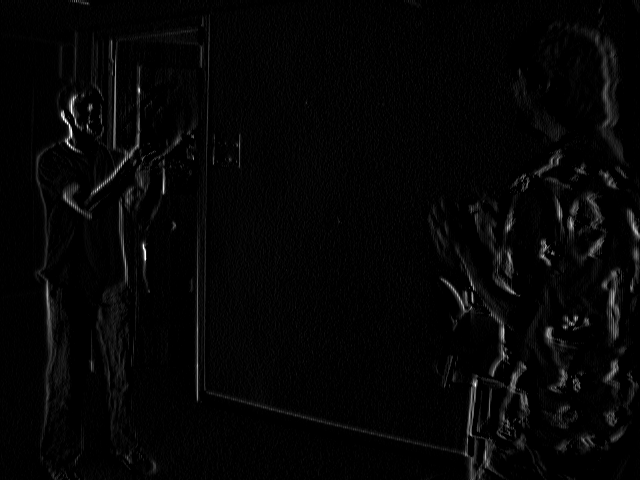
\includegraphics[width=0.8\textwidth]{Basketball/img_x}
      \caption{$I_x$}
    \end{subfigure}
    \begin{subfigure}{0.5\textwidth}
      \centering
      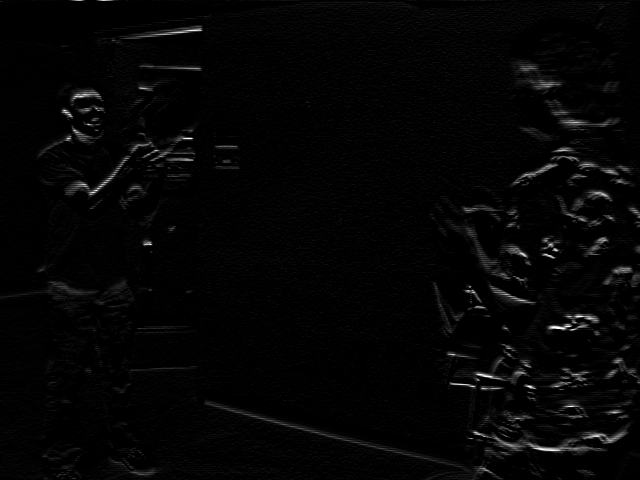
\includegraphics[width=0.8\textwidth]{Basketball/img_y}
      \caption{$I_y$}
    \end{subfigure}
     \begin{subfigure}{\textwidth}
      \centering
      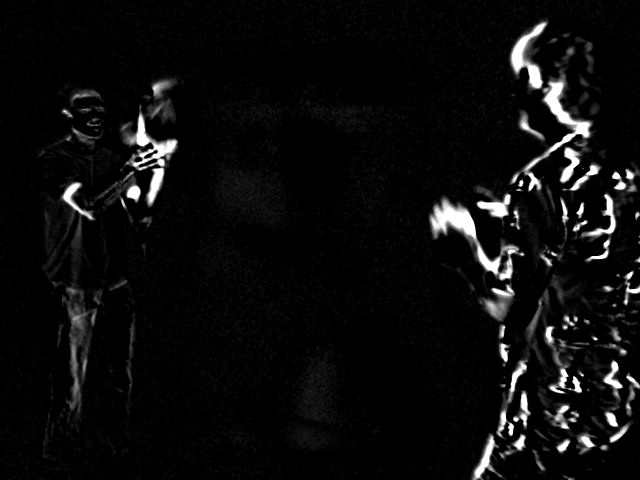
\includegraphics[width=0.4\textwidth]{Basketball/img_t}
      \caption{$I_t$}
    \end{subfigure}
  \end{figure}

  \subsection{Solving for $v_x, v_y$}
  
  Once the gradients are estimated, we form our linear system of equations of the form $Av = b$, where
  
  \begin{figure}[H]
  \centering
  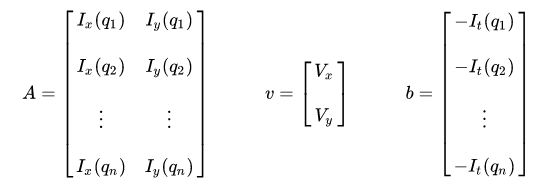
\includegraphics[scale=0.4]{avb}
  \end{figure}
  
  
  Applying least-squares, we get
  
  \begin{figure}[H]
   \centering
   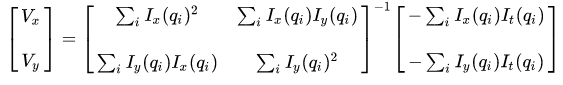
\includegraphics[scale=0.4]{inverse}
  \end{figure}

  In code, this is implemented as follows:
  
  \begin{lstlisting}[language=C++]
  
std::vector<float> OpticalFlow::getWindow(const cv::Mat &mat, const int &i, const int &j)
{
	std::vector<float> window;
	for(size_t ii = i - window_size/2; ii <= i + window_size/2; ii++)
		for(size_t jj = j - window_size/2; jj <= j + window_size/2; jj++)
		{
			window.push_back(mat.at<float>(ii, jj));
		}

	return window;
}

cv::Mat OpticalFlow::sumOverWindow(const cv::Mat &mat)
{
    cv::Mat sum = cv::Mat::zeros(mat.size(), CV_32FC1);
    
    for(int i = window_size/2; i < mat.rows - window_size/2; i++)
        for(int j = window_size/2; j < mat.cols - window_size/2; j++)
        {
            std::vector<float> window = getWindow(mat, i, j);
            sum.at<float>(i, j) = std::accumulate(window.begin(), window.end(), 0.0);
        }
        
    return sum;        
}
void OpticalFlow::computeOpticalFlow(cv::Mat &u, cv::Mat &v)
{
    computeImageGradients();
    
    cv::Mat img_xx = img_x.mul(img_x);
    cv::Mat img_yy = img_y.mul(img_y);
    cv::Mat img_xy = img_x.mul(img_y);
    cv::Mat img_xt = img_x.mul(img_t);
    cv::Mat img_yt = img_y.mul(img_t);
    
    cv::Mat sum_img_xx = sumOverWindow(img_xx);
    cv::Mat sum_img_yy = sumOverWindow(img_yy);
    cv::Mat sum_img_xy = sumOverWindow(img_xy);
    cv::Mat sum_img_xt = sumOverWindow(img_xt);
    cv::Mat sum_img_yt = sumOverWindow(img_yt);
    
    cv::Mat tmp = sum_img_xx.mul(sum_img_yy) - sum_img_xy.mul(sum_img_xy);
    u = sum_img_xy.mul(sum_img_yt) - sum_img_yy.mul(sum_img_xt);
    v = sum_img_xt.mul(sum_img_xy) - sum_img_xx.mul(sum_img_yt);
    
    cv::divide(u, tmp, u);
    cv::divide(v, tmp, v);
}
  \end{lstlisting}
  \vspace{1em}
  
  \subsection{Results}
\begin{figure}[H]
  \begin{subfigure}{0.5\textwidth}
   \centering
   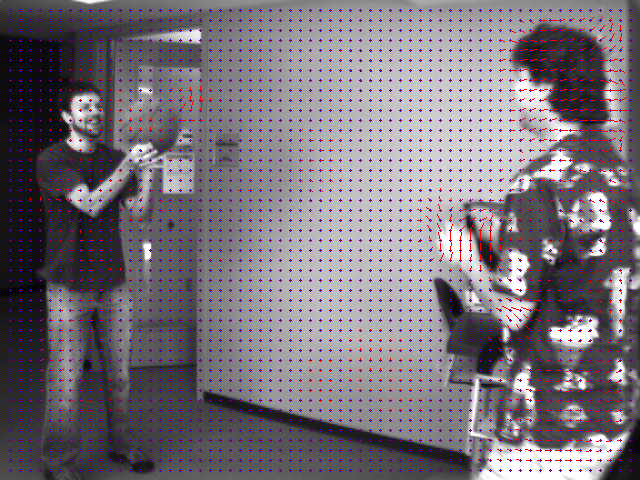
\includegraphics[width=0.8\linewidth]{Basketball/result_31x31.png}
  \end{subfigure}
  \begin{subfigure}{0.5\textwidth}
   \centering
   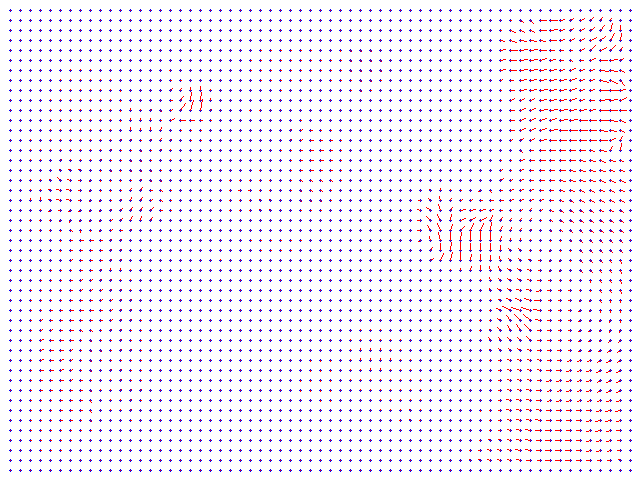
\includegraphics[width=0.8\linewidth]{Basketball/flow_31x31.png}
  \end{subfigure}
  \vspace{1em}
  
  \begin{subfigure}{0.5\textwidth}
   \centering
   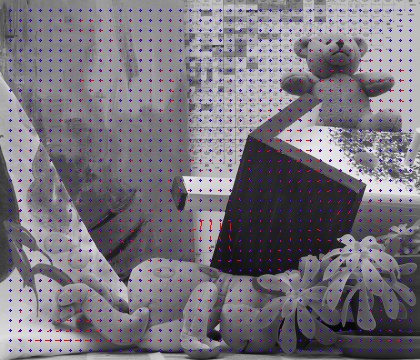
\includegraphics[width=0.8\linewidth]{Teddy/result_31x31.png}
   \end{subfigure}
   \begin{subfigure}{0.5\textwidth}
    \centering
    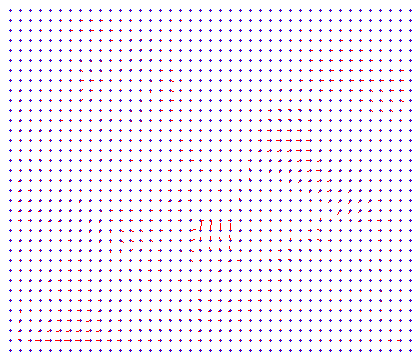
\includegraphics[width=0.8\linewidth]{Teddy/flow_31x31.png}
   \end{subfigure} 
     
     \end{figure}
     
    
    \begin{figure}[H]\ContinuedFloat
  \begin{subfigure}{0.5\textwidth}
   \centering
   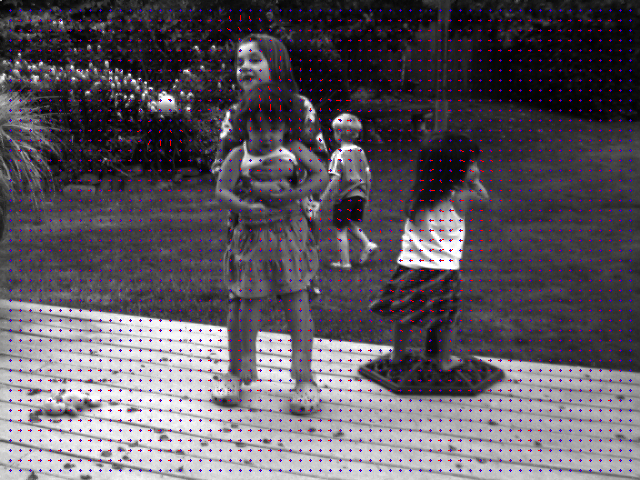
\includegraphics[width=0.8\linewidth]{Backyard/result_31x31.png}
   \end{subfigure}
   \begin{subfigure}{0.5\textwidth}
    \centering
    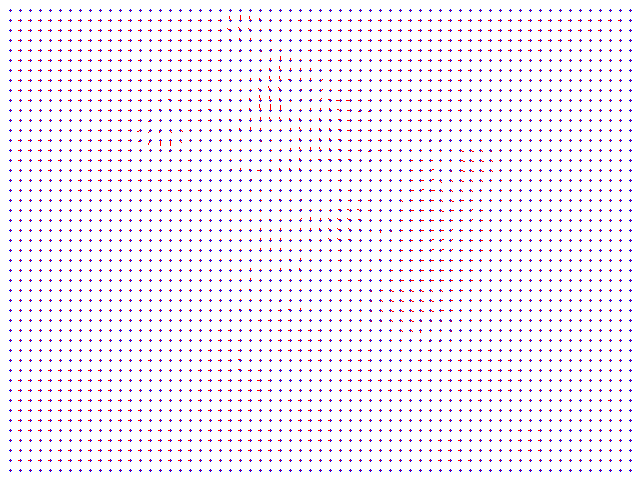
\includegraphics[width=0.8\linewidth]{Backyard/flow_31x31.png}
   \end{subfigure}
     \vspace{1em}
   
  \begin{subfigure}{0.5\textwidth}
   \centering
   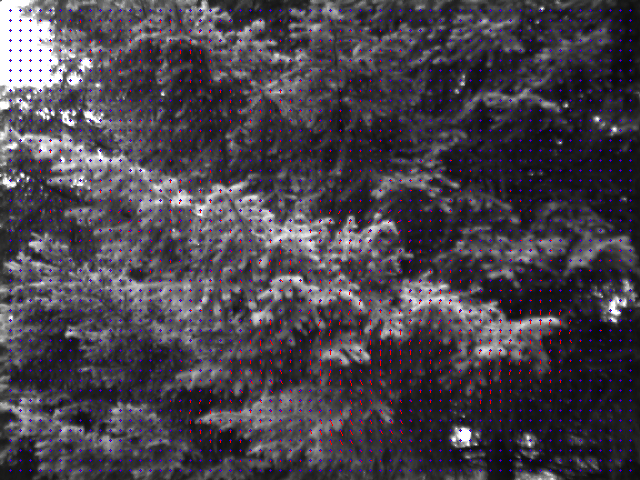
\includegraphics[width=0.8\linewidth]{Evergreen/result_31x31.png}
   \end{subfigure}
   \begin{subfigure}{0.5\textwidth}
    \centering
    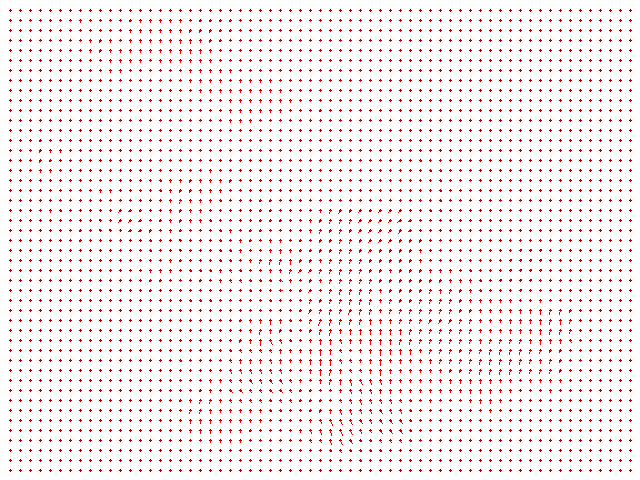
\includegraphics[width=0.8\linewidth]{Evergreen/flow_31x31.png}
   \end{subfigure}
     \vspace{1em}
   
  \begin{subfigure}{0.5\textwidth}
   \centering
   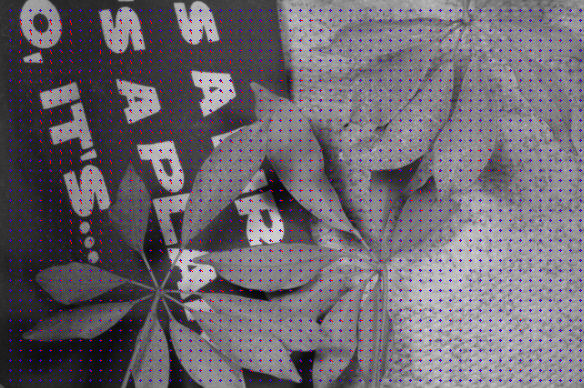
\includegraphics[width=0.8\linewidth]{Schefflera/result_31x31.png}
   \end{subfigure}
   \begin{subfigure}{0.5\textwidth}
    \centering
    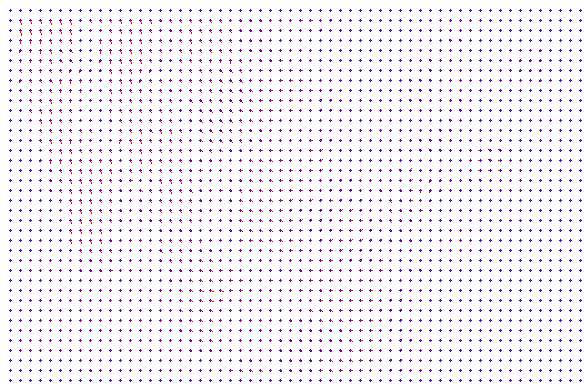
\includegraphics[width=0.8\linewidth]{Schefflera/flow_31x31.png}
   \end{subfigure}
   
   
  \caption{Blue dots indicate intial location, red lines indicate motion. The images (in order) are from the \texttt{Basketball, Teddy, Backyard, Evergreen, and Schefflera} sequences respectively.}
 
\end{figure}
  
     
\subsection{Observations}
\subsubsection*{Window size}

As the window size increases, the flow estimates are more consistent. For $3\times3$ size, the flow estimates are most noisy where as for $31\times31$ size they are most consistent.

\begin{figure}[H]
  \begin{subfigure}{0.5\textwidth}
   \centering
   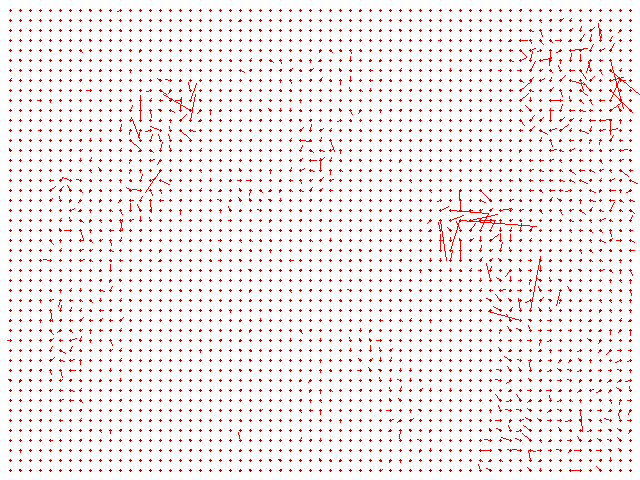
\includegraphics[width=0.8\linewidth]{Basketball/flow_3x3.png}
   \caption{$3 \times 3$}
  \end{subfigure}
  \begin{subfigure}{0.5\textwidth}
   \centering
   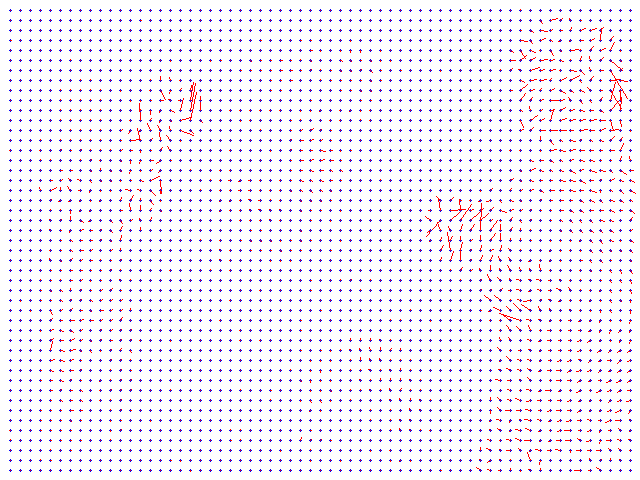
\includegraphics[width=0.8\linewidth]{Basketball/flow_7x7.png}
   \caption{$7 \times 7$}
  \end{subfigure}
  \end{figure}
  \begin{figure}[H]\ContinuedFloat
  \begin{subfigure}{0.5\textwidth}
   \centering
   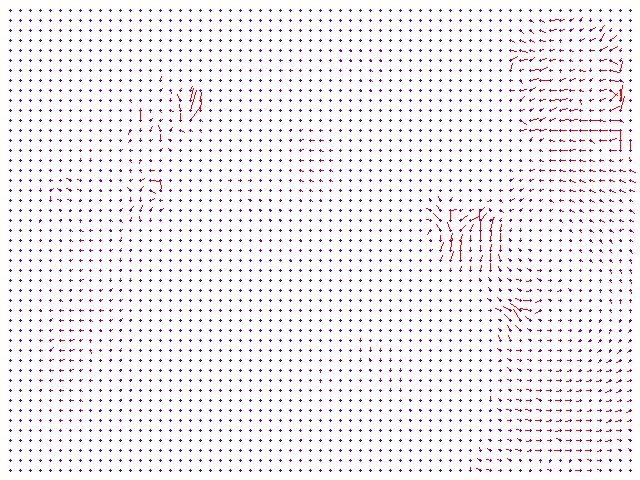
\includegraphics[width=0.8\linewidth]{Basketball/flow_15x15.png}
   \caption{$15 \times 15$}
   \end{subfigure}
   \begin{subfigure}{0.5\textwidth}
    \centering
    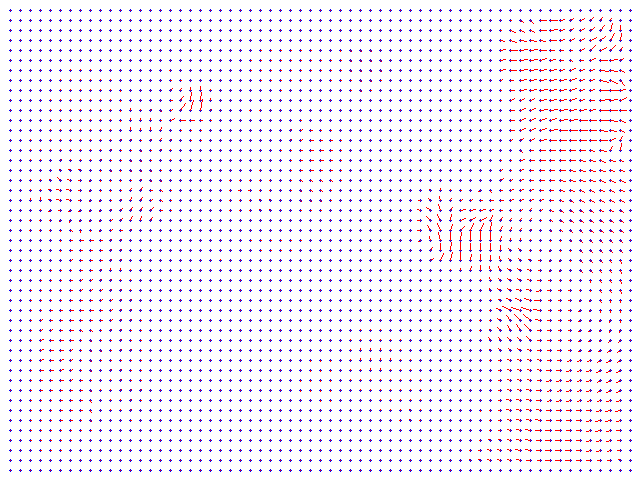
\includegraphics[width=0.8\linewidth]{Basketball/flow_31x31.png}
    \caption{$31 \times 31$}
   \end{subfigure}
  \caption{Effect of different window sizes on the \texttt{Basketball} sequence.}
\end{figure}

As expected, the run time increases by a factor of almost $3$ when the window size is doubled.

  \begin{center}
   \begin{tabular}{|c|c|c|c|}
      \hline
      \textbf{Size} & Time elapsed\\
      \hline
      $3 \times 3$& 2.17 s\\
      \hline
      $7 \times 7$ & 4.74 s\\
      \hline
      $15 \times 15$ & 12.21 s\\
      \hline
      $31 \times 31$ & 38.50 s\\
      \hline
   \end{tabular}
   \end{center}
   
   \subsubsection*{Sparse optical flow}
   
   Instead of computing optical flow for every pixel in the image, we can compute the flow only for ``good'' features. These are features for which the second moment matrix has large and relatively similar eigen values. This is the basis of the Kanade-Lucas-Tomasi feature tracker. However this could not be implemented completely for this assignment.
   
   \subsubsection*{Iterative LK, Hierarchial LK}
    LK optical flow is based on the fundamental assumption that motion is small. However this need not be the case since motion can be large and nonlinear. To handle such scenarios, an iterative version of LK can be applied. LK is also susceptible to local minima, which can be handled by applying a hieararchial (coarse-to-fine) approach.
   
   \subsection*{Camera motion}
   
   Optical flow is the relative motion between the objects in the scene and the camera, so when there is camera motion it appears as flow as well. The \texttt{Backyard} sequence is one example where there's camera motion. This is undesireable in motion detection applications, while desirable in image stabilization applications.


\section{Motion segmentation}

After optical flow computation, motion segmentation can be carried out by thresholding and then separating the optical flow vectors based on magnitude and direction. One way to do this is as follows,

\begin{lstlisting}[language=C++]
void drawMotionSeg(cv::Mat &u, cv::Mat &v)
{
    cv::Mat mag, angle;
    cv::cartToPolar(u, v, mag, angle);
    
    for(int i = 0; i < u.rows; i++)
        for(int j = 0; j < u.cols; j++)
        {
            if(u.at<float>(i, j) < 50)
                u.at<float>(i, j) = 0;
            
            else if(v.at<float>(i, j) < 50)
                v.at<float>(i, j) = 0;
        }
    
    cv::Mat hsv = cv::Mat::zeros(u.size(), CV_8UC3);
    
    for(int i = 0; i < u.rows; i++)
        for(int j = 0; j < v.cols; j++)
        {
            cv::Vec3b value;
            value[0] = 2 * angle.at<float>(i, j) * 180 / 3.14;
            value[1] = 255;
            value[2] = mag.at<float>(i, j) * 255; 
            hsv.at<cv::Vec3b>(i, j) = value;
        }
    
    cv::Mat bgr;
    cv::cvtColor(hsv, bgr, CV_HSV2BGR);
    cv::namedWindow("motion", CV_WINDOW_NORMAL);
    cv::imshow("motion", bgr);
    cv::waitKey(0);
}
\end{lstlisting}

\begin{figure}[H]
  \begin{subfigure}{0.5\textwidth}
    \centering
    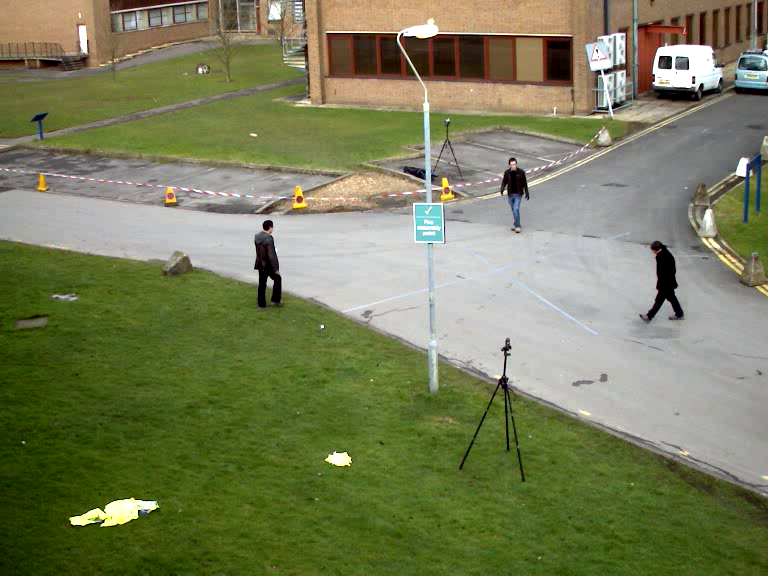
\includegraphics[width=0.8\linewidth]{frame}
    \caption{Input frame}
  \end{subfigure}
  \begin{subfigure}{0.5\textwidth}
    \centering
    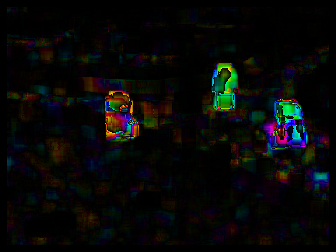
\includegraphics[width=0.8\linewidth]{motion_seg}
    \caption{Motion segmentation}
  \end{subfigure}
\end{figure}


\section{Object tracking}

For object tracking, an object of interest is first selected by the user by drawing a bounding box. Then the mean flow within the bounding box is used to update the location of the box in the subsequent frames. However this approach failed to work reliably and the object was lost track of after 6 frames as shown.

 \begin{figure}[H]
  \begin{subfigure}{0.5\textwidth}
   \centering
   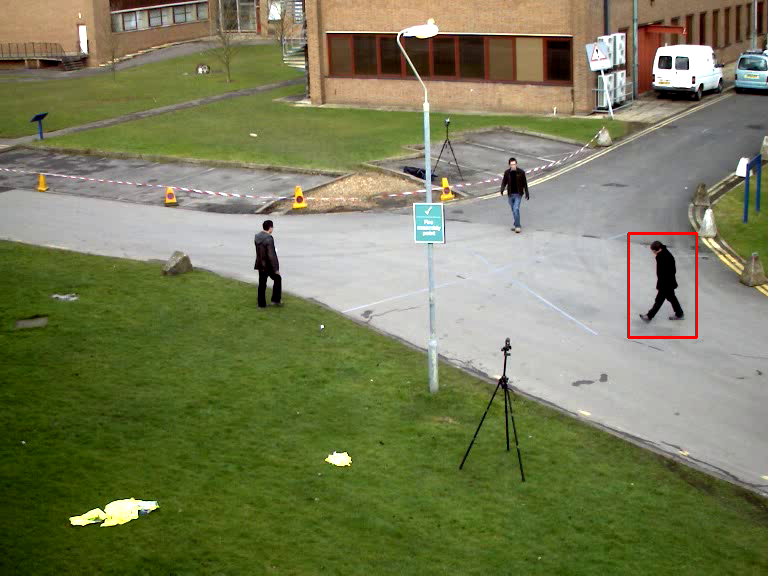
\includegraphics[width=0.8\linewidth]{first.png}
   \caption{First frame with user selection}
  \end{subfigure}
  \begin{subfigure}{0.5\textwidth}
   \centering
   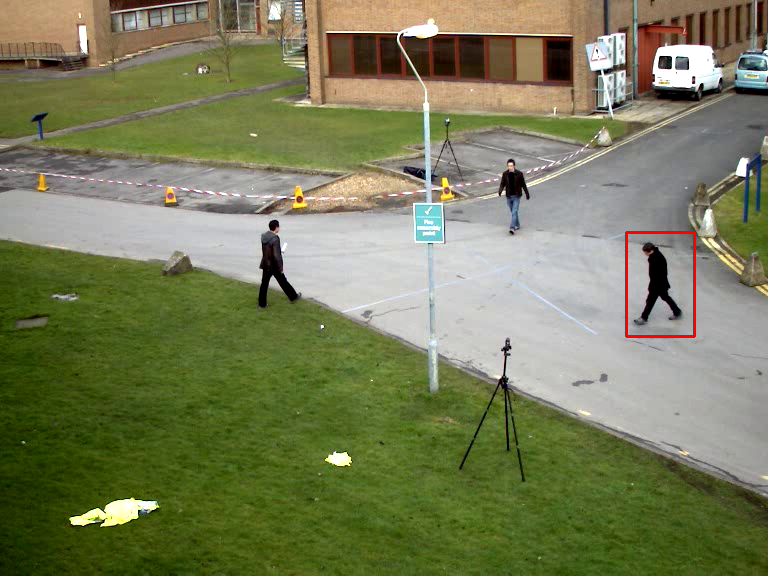
\includegraphics[width=0.8\linewidth]{track1.png}
   \caption{Track 1}
  \end{subfigure}
  \vspace{1em}
  
  \begin{subfigure}{0.5\textwidth}
   \centering
   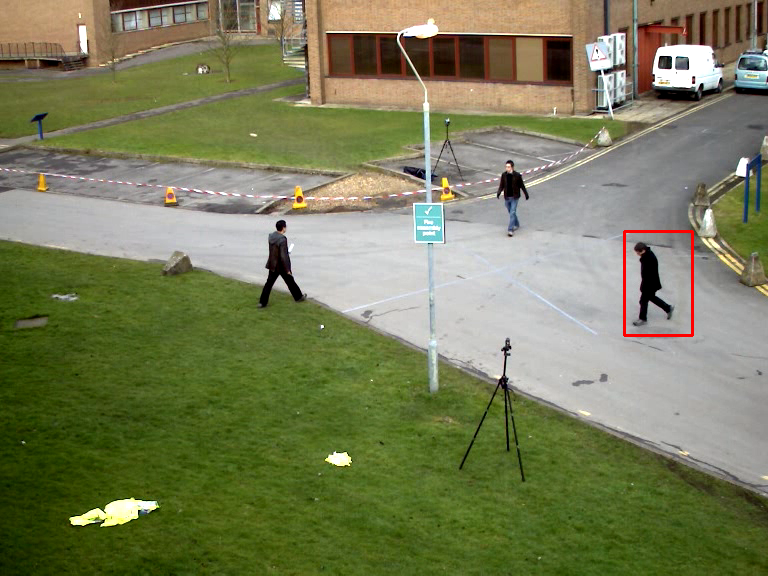
\includegraphics[width=0.8\linewidth]{track2.png}
   \caption{Track 2}
   \end{subfigure}
   \begin{subfigure}{0.5\textwidth}
    \centering
    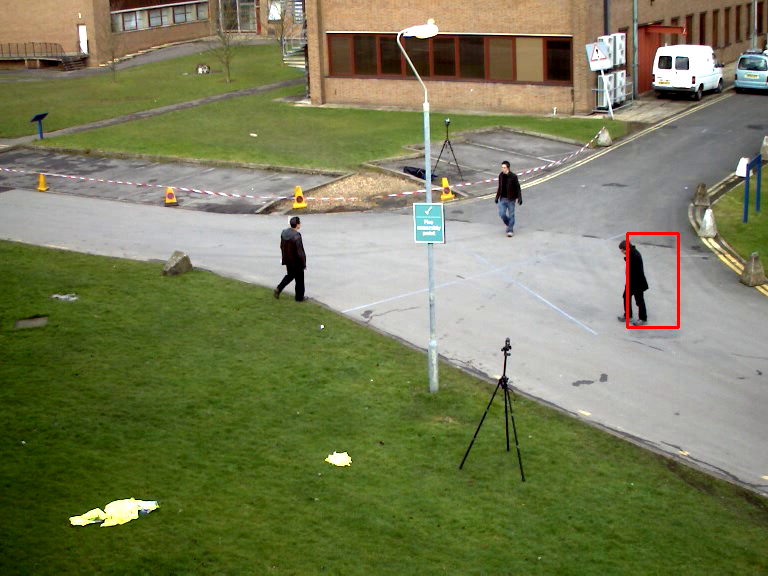
\includegraphics[width=0.8\linewidth]{track3.png}
    \caption{Track 3}
   \end{subfigure} 
   \end{figure}
    
    \begin{figure}[H]\ContinuedFloat
  \begin{subfigure}{0.5\textwidth}
   \centering
   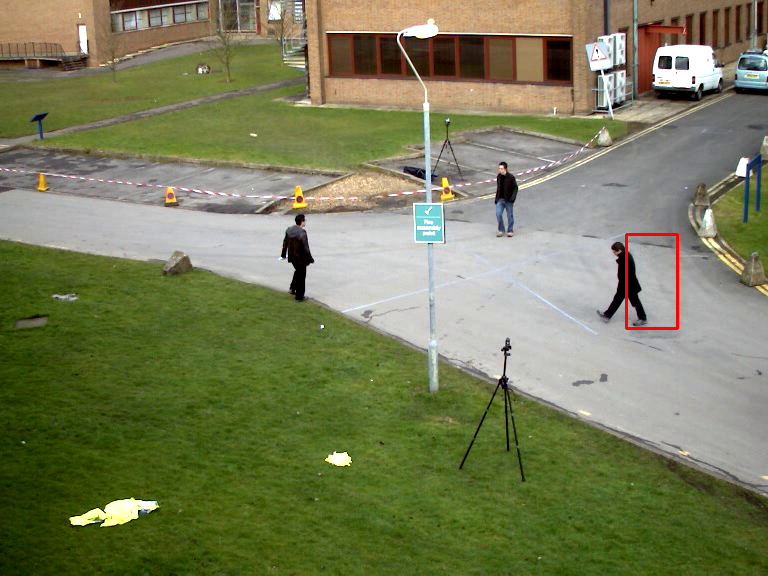
\includegraphics[width=0.8\linewidth]{track4.png}
   \caption{Track 4}
   \end{subfigure}
   \begin{subfigure}{0.5\textwidth}
    \centering
    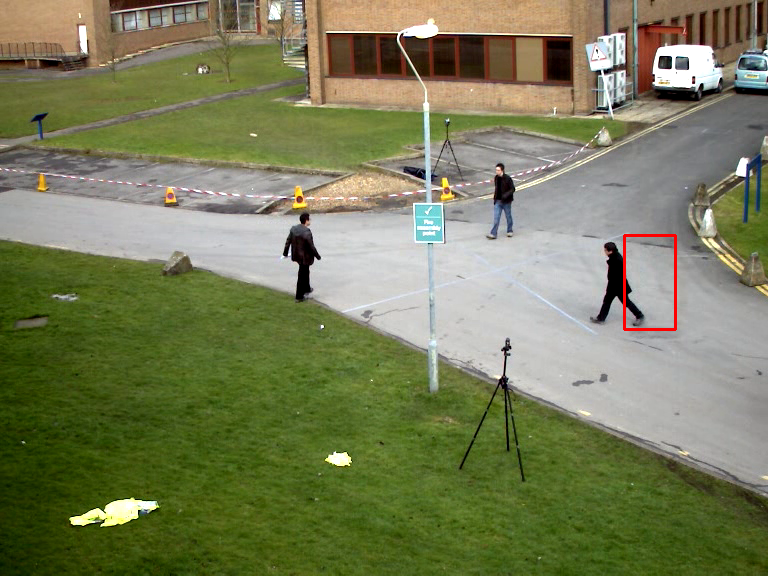
\includegraphics[width=0.8\linewidth]{track5.png}
    \caption{Track 5}
   \end{subfigure}
     \vspace{1em}
   
  \begin{subfigure}{0.5\textwidth}
   \centering
   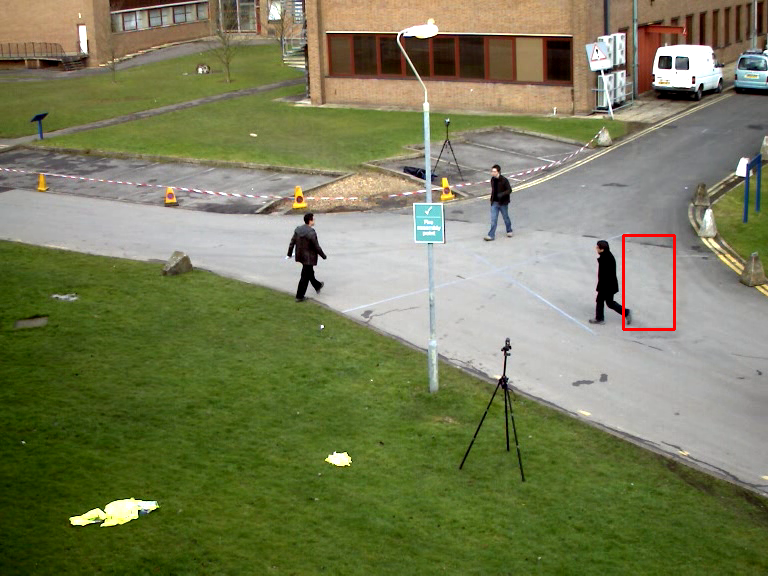
\includegraphics[width=0.8\linewidth]{track6.png}
   \caption{Track 6}
   \end{subfigure}
   \begin{subfigure}{0.5\textwidth}
    \centering
    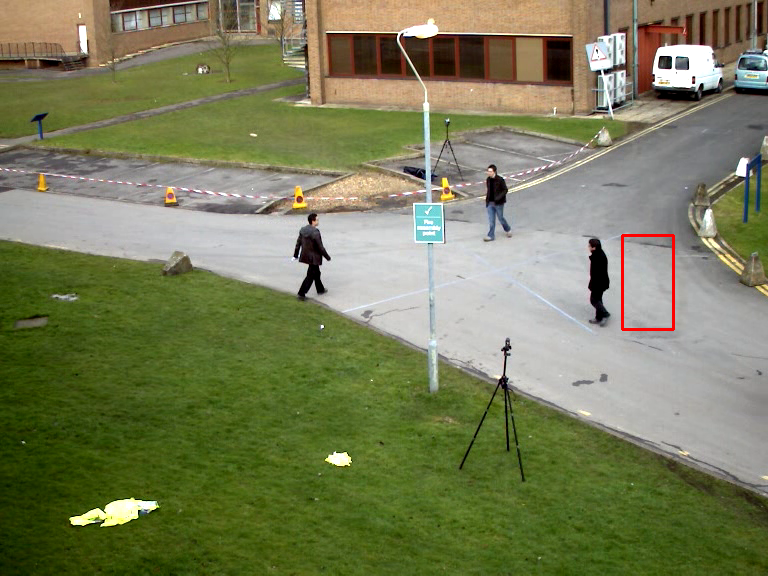
\includegraphics[width=0.8\linewidth]{track7.png}
    \caption{Track 7}
   \end{subfigure}
   
\end{figure}

Some immediate improvements that can be tried next - use median instead of mean flow since the mean flow is almost zero (but computing median is expensive), use iterative LK to deal with nonlinear motion, and use hierarchial LK to handle large motion.

\end{document}
